\chapter{Architecture et Réalisation du Sprint 1}
\label{chap:architecture_sprint1}

\section{Introduction}
Après avoir rigoureusement défini le périmètre fonctionnel et les exigences du projet dans le chapitre précédent, nous entrons à présent dans la phase de conception technique et de réalisation. La transition d'un processus manuel dispersé vers une plateforme web centralisée exige des fondations logicielles solides, capables de soutenir la montée en charge, d'assurer la sécurité des données industrielles, et de faciliter les évolutions futures. Ce troisième chapitre est dédié à la mise en place de ces fondations. Dans un premier temps, nous justifierons en détail l'ensemble des choix technologiques adoptés, en confrontant les besoins du Groupe COFAT aux standards actuels de l'industrie logicielle. Nous décrirons ensuite l'architecture 3-tiers mise en œuvre ainsi que le diagramme de déploiement physique. Enfin, nous aborderons la phase de réalisation concrète en présentant les travaux du Sprint 0 (mise en place du socle technique) et du Sprint 1, qui a donné naissance au module d'authentification sécurisé et au tableau de bord d'administration central, pierres angulaires de l'application \textit{Cofat Capacity Study}.

\section{Choix technologiques}
La sélection de la \textit{stack} technique (l'empilement des technologies) est une décision critique. Elle doit répondre aux exigences non fonctionnelles de sécurité, de performance lors de l'agrégation de milliers de données, et de maintenabilité par les futures équipes IT de COFAT. Nous avons opté pour une approche \textit{Full-Stack JavaScript} accompagnée d'une base de données relationnelle robuste.

Ce choix d'un langage unique (JavaScript/Node.js) pour l'ensemble de la pile applicative, plutôt qu'une combinaison hétérogène de technologies différentes pour le frontend et le backend, répond à une contrainte concrète du contexte de ce PFE : le développement a été assuré par une équipe technique réduite (le stagiaire développeur, épaulé ponctuellement par le Scrum Master), sans possibilité de spécialiser des ressources distinctes par couche technique. L'homogénéité du langage réduit la charge cognitive lors du passage d'un fichier frontend à un fichier backend, accélère la montée en compétence, et facilite le partage de structures de données (par exemple, la validation d'un objet JSON peut réutiliser des schémas très proches côté client et côté serveur). Ce choix facilite également la passation du projet à l'équipe IT d'ABM Informatique à l'issue du stage, celle-ci n'ayant besoin de maîtriser qu'un seul écosystème technique plutôt que deux.

\subsection{Environnement Backend : Node.js et Express.js}
\textbf{Définition :} Node.js est un environnement d'exécution (runtime) open-source multiplateforme qui permet d'exécuter du code JavaScript côté serveur. Il repose sur le moteur V8 de Google Chrome et utilise une architecture asynchrone non bloquante orientée événements (Event Loop). Express.js est le framework web minimaliste et flexible le plus populaire pour Node.js.
\newline
\textbf{Raison du choix :} Le besoin principal du backend de \textit{Cofat Capacity Study} est de traiter des requêtes entrantes (imports de gros fichiers Excel) et de servir des données consolidées simultanément à plusieurs usines mondiales. L'asynchronisme natif de Node.js est particulièrement adapté aux opérations d'entrées/sorties (I/O) intensives sans bloquer le thread principal. L'utilisation du JavaScript de bout en bout (frontend et backend) homogénéise le code et facilite la maintenance.
\newline
\textbf{Utilisation dans le projet :} Le serveur Node.js/Express héberge notre API RESTful. Il écoute sur le port \textbf{9001}. L'architecture est modulaire, avec un routage organisé par domaine métier (authentification, équipements, espaces, RH, budget). Express gère les middlewares globaux (sécurité CORS, parsing JSON, gestion des erreurs) et les requêtes HTTP.

\subsection{Système de Gestion de Base de Données : Microsoft SQL Server}
\textbf{Définition :} Microsoft SQL Server (MSSQL) est un système de gestion de base de données relationnelle (SGBDR) d'entreprise, reconnu pour sa fiabilité, ses capacités transactionnelles (ACID) et ses performances sur de gros volumes de données.
\newline
\textbf{Raison du choix :} Le modèle de données de COFAT est intrinsèquement relationnel : une usine possède plusieurs équipements, qui sont liés à des périodes de planification, tandis qu'un budget est rattaché à un historique de notifications. Une base NoSQL n'aurait pas été adaptée pour garantir l'intégrité de ces liens via des clés étrangères. Par ailleurs, MS SQL Server est le standard SGBDR historique et validé par le département IT d'ABM Informatique (la branche IT du groupe), ce qui facilite l'intégration dans leur infrastructure existante.
\newline
\textbf{Utilisation dans le projet :} La base de données, nommée \texttt{GALIA\_V1}, est hébergée sur l'instance SQL Server de l'entreprise et communique sur le port standard \textbf{1433}. Elle stocke de manière sécurisée l'ensemble des 10 entités de l'application.

\subsection{Object-Relational Mapping (ORM) : Sequelize}
\textbf{Définition :} Sequelize est un ORM (Object-Relational Mapper) basé sur des promesses pour Node.js, supportant de nombreux dialectes SQL dont MSSQL.
\newline
\textbf{Raison du choix :} Rédiger des requêtes SQL "brutes" dans le code backend expose aux risques d'injection SQL et rend la maintenance fastidieuse. Sequelize permet de manipuler les tables de la base de données comme des objets JavaScript classiques. Il gère automatiquement l'assainissement des données et facilite les migrations de schémas.
\newline
\textbf{Utilisation dans le projet :} Chaque table SQL est représentée par un modèle JavaScript dans le dossier \texttt{models/}. Sequelize est utilisé pour définir les champs (avec leurs validations de type strictes) et les relations (\textit{hasMany}, \textit{belongsTo}). Ses méthodes (\textit{findAll}, \textit{bulkCreate}) sont massivement utilisées pour la consolidation et l'import Excel.

\textbf{Protection contre l'injection SQL :} l'un des bénéfices de sécurité les plus concrets de l'usage systématique de Sequelize, plutôt que de requêtes SQL concaténées manuellement, réside dans la paramétrisation automatique de toutes les requêtes générées par l'ORM. Lorsqu'un Site Manager saisit une valeur dans un champ de recherche ou de filtre (par exemple le nom d'un projet client dans le module Espaces), cette valeur est systématiquement transmise à la base de données comme un paramètre distinct de la requête SQL elle-même, plutôt que d'être insérée directement dans le texte de la requête. Cette pratique élimine par construction toute possibilité d'injection SQL malveillante, une classe de vulnérabilité particulièrement critique à prévenir dans une application manipulant des données financières et stratégiques sensibles comme celles de \textit{Cofat Capacity Study}.

\subsection{Environnement Frontend : React.js}
\textbf{Définition :} React.js est une bibliothèque JavaScript open-source développée par Facebook (Meta) pour la création d'interfaces utilisateur interactives sous forme de Single Page Application (SPA).
\newline
\textbf{Raison du choix :} React permet de créer des interfaces réactives et modulaires basées sur des composants réutilisables. Son concept de DOM virtuel (Virtual DOM) offre des performances d'affichage exceptionnelles, idéales pour manipuler les vastes tableaux de bord de consolidation de COFAT sans avoir à recharger la page.
\newline
\textbf{Utilisation dans le projet :} Le frontend est entièrement développé en React avec des composants fonctionnels (Functional Components) et les Hooks (\textit{useState}, \textit{useEffect}). L'API Context de React est utilisée pour maintenir l'état d'authentification global de l'utilisateur à travers toutes les pages.

\subsection{Bibliothèques d'interface (UI) : Tailwind CSS, MUI, Ant Design}
\textbf{Définitions et Raisons du choix :} L'ergonomie est une priorité. 
\begin{itemize}
    \item \textbf{Tailwind CSS} est un framework CSS \textit{utility-first}. Contrairement aux frameworks basés sur des composants (comme Bootstrap), Tailwind permet d'appliquer des styles directement dans le code JSX via des classes utilitaires. Cela permet de créer un design totalement sur mesure et \textit{responsive} (adaptable PC/Tablette) sans s'alourdir de lourds fichiers CSS, ni recourir aux fastidieuses media queries.
    \item \textbf{Material UI (MUI)} et \textbf{Ant Design (AntD)} sont des bibliothèques de composants React prêts à l'emploi. 
\end{itemize}
\textbf{Utilisation :} Tailwind est utilisé pour structurer les mises en page (Grid, Flexbox) et les couleurs du thème (Dark Mode, palettes harmonieuses). MUI et Ant Design sont déployés de manière chirurgicale pour les composants complexes tels que les tableaux de données massifs (DataTables), les modales de confirmation, et les formulaires interactifs.

\textbf{Pourquoi coexistence de trois bibliothèques UI plutôt qu'une seule ?} Ce choix, qui pourrait à première vue sembler redondant, répond en réalité à une répartition précise des responsabilités entre les trois outils. Tailwind CSS gère exclusivement la mise en page globale et l'identité visuelle (espacements, couleurs, typographie), tandis que MUI est privilégié pour les composants nécessitant une accessibilité clavier robuste et une gestion fine des états de formulaire (champs de saisie, sélecteurs de date), et Ant Design pour ses composants de tableaux de données particulièrement adaptés à l'affichage de matrices complexes comme celles du module RH (chapitre 4). Plutôt que de développer ces composants complexes à la main avec Tailwind seul, ce qui aurait représenté un investissement en temps considérable pour un projet de fin d'études aux délais contraints, la réutilisation de composants déjà éprouvés par ces deux bibliothèques a permis de concentrer l'effort de développement sur la logique métier propre à COFAT plutôt que sur la réinvention de briques d'interface génériques déjà résolues par la communauté open-source.

\subsection{Visualisation de données : Charts.js}
\textbf{Définition :} Charts.js est une bibliothèque JavaScript permettant de dessiner des graphiques dynamiques sur un élément Canvas HTML5.
\newline
\textbf{Raison du choix :} L'application nécessite de traduire visuellement la capacité de production pour faciliter la prise de décision.
\newline
\textbf{Utilisation :} Utilisée pour générer les graphiques d'analyse d'occupation des espaces (diagrammes circulaires) et les courbes d'évolution des effectifs (histogrammes et lignes de tendance) sur les tableaux de bord de consolidation "Cofat Group".

\subsection{Outils de Modélisation et de Développement}
\begin{itemize}
    \item \textbf{PlantUML} : Outil open-source permettant de générer des diagrammes UML de haute qualité à partir d'un langage de description textuel. Utilisé pour toute la modélisation conceptuelle de ce rapport.
    \item \textbf{Visual Studio Code (VS Code)} : L'éditeur de code (IDE) principal, léger et puissant. Les extensions "ES7+ React/Redux/React-Native snippets" ont drastiquement accéléré l'écriture des composants.
\end{itemize}

\subsection{Contrôle de version et gestion du code : Git}
Pour assurer un cycle de développement professionnel et sécurisé :
\begin{itemize}
    \item \textbf{Git} : Utilisé pour le \textit{versioning} du code source tout au long des quatre sprints du projet. La méthodologie \textit{Git Flow} a été appliquée, avec des branches dédiées pour chaque nouvelle fonctionnalité (\textit{feature branches}) afin de ne jamais compromettre le code stable de la branche principale lors du développement de nouvelles fonctions.
    \item \textbf{Fichier \texttt{.gitignore}} : Les fichiers sensibles (\texttt{.env}, \texttt{node\_modules/}) sont systématiquement exclus du dépôt, garantissant qu'aucune configuration d'environnement de production ne soit exposée dans l'historique Git.
\end{itemize}

\section{Architecture 3-tiers de l'application}
Pour répondre aux impératifs d'extensibilité et de maintenabilité, l'application repose sur une architecture logique à trois niveaux (3-tiers). Ce modèle sépare physiquement et logiquement l'interface utilisateur de la logique métier et du stockage des données, ce qui permet à chaque couche d'évoluer de manière indépendante.

\subsection{Couche de Présentation (Frontend - React)}
C'est l'interface avec laquelle les utilisateurs de COFAT interagissent. Elle a pour seule responsabilité l'affichage des informations et la capture des saisies utilisateurs. Elle ne contient aucune règle métier complexe.
\newline
\textbf{Composants principaux :} Le frontend est composé de vues (Pages) et de fragments réutilisables (Components). Parmi les composants réels de l'application, on retrouve :
\begin{itemize}
    \item \textit{Login} : Écran d'authentification.
    \item \textit{AdminDashboard} : Interface centrale réservée à la direction.
    \item \textit{SiteTable}, \textit{SpaceTable}, \textit{HrTable} : Tableaux de gestion de la planification locale.
    \item \textit{CofatGroup} : Composants de consolidation mondiale.
    \item \textit{NonIndustrialBudget} et \textit{StandardInvestment} : Vues de gestion financière.
    \item \textit{NotificationBell} : Composant global interrogeant l'API pour afficher les alertes.
\end{itemize}

\subsection{Couche Métier (Backend - Node.js/Express)}
C'est le cerveau de l'application. Elle reçoit les requêtes de la couche de présentation via HTTP, exécute les règles de gestion (calculs de capacité, validations des permissions) et communique avec la base de données.
\newline
\textbf{Gestion des middlewares et sécurité :} Chaque requête passe d'abord par le middleware de sécurité JWT. Ce script intercepte la requête, extrait le cookie \textit{HttpOnly}, décrypte la signature du jeton, vérifie l'identité de l'utilisateur et s'assure qu'il possède le rôle requis (\textit{Admin}, \textit{Site Manager}, ou \textit{Achat}) avant de l'autoriser à exécuter la logique de la route.

Le tableau \ref{tab:api_endpoints} présente un extrait représentatif des API REST développées pour ce projet.

\begin{table}[h]
\centering
\begin{tabular}{|p{2.5cm}|p{6cm}|p{4.5cm}|p{2cm}|}
\hline
\textbf{Méthode HTTP} & \textbf{Route API} & \textbf{Description} & \textbf{Rôle requis} \\ \hline
POST & \texttt{/signin} & Authentifie l'utilisateur, crée le cookie JWT & Tous \\ \hline
GET & \texttt{/api/sites} & Liste les sites COFAT & Admin \\ \hline
POST & \texttt{/api/equipment-planning/import} & Parse et insère le fichier Excel Équipements & Site Mgr \\ \hline
GET & \texttt{/api/space} & Récupère les espaces d'un site & Site Mgr \\ \hline
GET & \texttt{/api/cofat-group} & Agrège les effectifs RH à l'échelle mondiale & Admin \\ \hline
PUT & \texttt{/api/standard-investments-v2/save} & Met à jour le coût d'un équipement de référence & Admin, Achat \\ \hline
GET & \texttt{/api/non-industrial-budget/search} & Recherche avec filtres dans le budget & Tous \\ \hline
POST & \texttt{/api/non-industrial-budget/create} & Crée une nouvelle ligne budgétaire & Site Mgr \\ \hline
PUT & \texttt{/api/non-industrial-budget/update/:id} & Modifie un budget (ex~: prix unitaire) & Site Mgr, Achat \\ \hline
DELETE & \texttt{/api/non-industrial-budget/delete/:id} & Supprime une ligne de budget & Site Mgr \\ \hline
GET & \texttt{/api/non-industrial-budget/notifications/unread} & Récupère les alertes non lues & Tous \\ \hline
PUT & \texttt{/api/non-industrial-budget/notifications/:id/read} & Marque une notification comme lue & Tous \\ \hline
\end{tabular}
\caption{Extrait des routes API REST principales de l'application}
\label{tab:api_endpoints}
\end{table}

\textbf{Conventions REST adoptées :} l'ensemble de l'API respecte une convention de nommage cohérente basée sur les ressources plutôt que sur les actions : les URLs désignent des noms (\texttt{/api/budget}, \texttt{/api/sites}) et c'est le verbe HTTP (GET, POST, PUT, DELETE) qui porte la sémantique de l'action à réaliser sur cette ressource. Cette approche, standard dans l'écosystème Express, facilite grandement l'onboarding de tout futur développeur rejoignant l'équipe IT d'ABM Informatique, puisque la structure des routes est prévisible et auto-documentée. Chaque contrôleur retourne systématiquement un objet JSON structuré contenant, en cas de succès, les données demandées, et en cas d'erreur, un code de statut HTTP approprié (400 pour une requête malformée, 401 pour une authentification manquante, 403 pour un rôle insuffisant, 404 pour une ressource introuvable, 500 pour une erreur serveur imprévue) accompagné d'un message d'erreur exploitable par le frontend React pour informer l'utilisateur.

\textbf{Gestion centralisée des erreurs :} plutôt que de dupliquer des blocs \texttt{try/catch} dans chaque contrôleur, un middleware d'erreur global a été positionné en fin de chaîne Express. Toute exception non interceptée localement remonte automatiquement vers ce gestionnaire central, qui journalise l'erreur côté serveur (utile pour le débogage en production) tout en renvoyant une réponse JSON générique et sécurisée au client, évitant ainsi d'exposer accidentellement des détails techniques sensibles (comme la structure interne d'une requête SQL) à un utilisateur final.


\subsection{Couche Données (SQL Server)}
Cette couche garantit la persistance, l'intégrité et la disponibilité des données. Elle est constituée de l'instance MS SQL Server, contenant la base \texttt{GALIA\_V1}. Cette base contient les tables physiques générées automatiquement par Sequelize à partir de nos 10 modèles (Users, Sites, NonIndustrialBudget, etc.).

\vspace{0.5cm}
\begin{figure}[H]
    \centering
    
\includegraphics[width=0.8\textwidth]{img/architecture.png}
    \caption{Architecture logicielle 3-tiers de l'application}
    \label{fig:architecture}
\end{figure}
\vspace{0.5cm}

\section{Diagramme de déploiement}
L'architecture physique (infrastructure) définit la manière dont les différents composants logiciels sont déployés sur le réseau de l'entreprise.

\vspace{0.5cm}
\begin{figure}[H]
    \centering
    
\includegraphics[width=0.9\textwidth]{img/Diagramme de déploiement.png}
    \caption{Diagramme de déploiement réseau de Cofat Capacity Study}
    \label{fig:deploiement}
\end{figure}
\vspace{0.5cm}

\textbf{Analyse de l'infrastructure réelle :} 
L'application est conçue pour fonctionner sur le réseau interne (Intranet) du Groupe COFAT pour des raisons évidentes de confidentialité.
\begin{itemize}
    \item \textbf{Poste Client} : Le Site Manager ou l'Acheteur utilise un navigateur web standard (Google Chrome ou Microsoft Edge). Le frontend React, servi initialement sur le port 4000 par le serveur web, s'exécute localement dans la mémoire du navigateur client.
    \item \textbf{Serveur d'Application (Node.js)} : Hébergé sur une machine virtuelle Linux via Docker chez ABM Informatique, l'API Express écoute les requêtes sur le port \textbf{9001}. Ce serveur possède également l'accès en écriture à deux répertoires de stockage : \texttt{/uploads/images} pour les photos des machines de référence, et \texttt{/uploads/budget} pour la sauvegarde temporaire des fichiers Excel importés avant leur traitement.
    \item \textbf{Serveur de Base de données (SQL Server)} : Hébergé sur un cluster sécurisé distinct de l'entreprise, écoutant sur le port TCP \textbf{1433}. Le serveur Express s'y connecte via des identifiants stockés dans des variables d'environnement (\texttt{.env}).
\end{itemize}

Ce cloisonnement en trois niveaux physiques distincts (poste client, serveur applicatif, serveur de données) répond à un principe de sécurité fondamental en environnement industriel : aucun poste client, même celui d'un Administrateur, n'établit de connexion directe avec la base de données SQL Server. Toute lecture ou écriture transite obligatoirement par la couche API Express, qui applique systématiquement les contrôles d'authentification et d'autorisation décrits précédemment. Cette architecture élimine par construction toute possibilité pour un utilisateur, même techniquement averti, d'accéder directement aux données brutes en contournant la logique applicative.

La communication entre le poste client et le serveur applicatif transite exclusivement par le protocole HTTP (et sa variante sécurisée HTTPS en environnement de production), tandis que la communication entre le serveur applicatif et le serveur de base de données utilise le protocole propriétaire TDS (Tabular Data Stream) de Microsoft, encapsulé par le driver \textit{tedious} évoqué au Sprint 0. Ce choix de séparation protocolaire renforce encore la défense en profondeur de l'infrastructure, chaque couche réseau n'exposant que les protocoles strictement nécessaires à son fonctionnement.


Ce cloisonnement réseau strict entre les trois couches (poste client, serveur applicatif, serveur de données) constitue une bonne pratique de sécurité fondamentale : le poste client ne dialogue jamais directement avec la base SQL Server, tout accès aux données transitant obligatoirement par l'API Express, seule habilitée à interroger la base via les identifiants stockés côté serveur. Un attaquant qui parviendrait à compromettre le poste d'un utilisateur ne pourrait donc, dans le pire des cas, qu'interagir avec l'API dans les limites du rôle de l'utilisateur compromis, sans jamais obtenir un accès direct au SGBD.

La variable d'environnement \texttt{.env}, non versionnée sur GitHub (exclue via \texttt{.gitignore}), centralise l'ensemble des paramètres sensibles : chaîne de connexion SQL Server, clé secrète de signature JWT, port d'écoute, et origine CORS autorisée pour le frontend. Cette séparation entre code source et configuration sensible, conforme aux principes de la méthodologie \textit{Twelve-Factor App} largement répandue dans l'industrie du logiciel, permet de déployer le même code sur plusieurs environnements (développement, production) sans jamais exposer de secret dans l'historique Git.


\section{Sprint 0 : Mise en place du socle technique}
Avant de coder la moindre interface utilisateur, la phase préparatoire du Sprint 0 s'est concentrée sur la création de la coquille vide de l'application et la configuration des dépendances npm essentielles.

\textbf{Côté Backend :}
Initialisation du projet Node via \texttt{npm init}, puis installation des briques logicielles :
\texttt{npm install express sequelize tedious cors dotenv bcryptjs jsonwebtoken cookie-parser multer xlsx}. 
(Note: le paquet \textit{tedious} est le driver de connexion officiel Microsoft pour SQL Server sous Node).
L'arborescence serveur a été structurée de manière professionnelle :
\begin{itemize}
    \item \texttt{/config} : Paramètres de base de données et clés secrètes.
    \item \texttt{/models} : Les 10 fichiers Sequelize définissant la BDD.
    \item \texttt{/routers} : Les points d'entrée des requêtes HTTP (ex: \texttt{nonIndustrialBudgetRoutes.js}).
    \item \texttt{/controllers} : La logique métier extraite des routes.
    \item \texttt{/middleware} : Scripts de vérification JWT et d'autorisation de rôles.
\end{itemize}

\textbf{Côté Frontend :}
Génération du \textit{boilerplate} React via \texttt{npx create-react-app}. Installation des outils visuels et réseaux :
\texttt{npm install react-router-dom axios tailwindcss @mui/material antd recharts}.
L'arborescence client :
\begin{itemize}
    \item \texttt{/components} : Les blocs d'interface réutilisables (Boutons, Modales, Navbar).
    \item \texttt{/pages} : Les vues entières assignées à des routes (ex: Dashboard).
    \item \texttt{/context} : Gestion globale de la session utilisateur.
    \item \texttt{/services} : Les scripts gérant les appels \textit{Axios} vers le port 9001 du backend.
\end{itemize}

\textbf{Rationale de la structuration en couches :} ce découpage en dossiers dédiés (\texttt{routers}/\texttt{controllers}/\texttt{middleware} côté serveur, \texttt{components}/\texttt{pages}/\texttt{services} côté client) suit le principe de responsabilité unique bien connu en génie logiciel : chaque fichier n'a qu'une seule raison de changer. Un routeur ne fait que déclarer les URLs et leur méthode HTTP associée, sans jamais contenir de logique métier ; un contrôleur ne fait qu'orchestrer la validation et l'appel aux modèles Sequelize, sans jamais gérer directement le format de la réponse HTTP brute. Cette discipline, adoptée dès le Sprint 0 avant même l'écriture de la première fonctionnalité métier, a grandement facilité le travail en parallèle : plusieurs modules (Équipements, Espaces, RH) ont pu être développés de façon quasi indépendante lors des sprints suivants, chacun ajoutant simplement son propre fichier dans les dossiers déjà structurés, sans jamais entrer en conflit avec le code existant des autres modules.

Ce même Sprint 0 a également été l'occasion de configurer les fichiers de variables d'environnement (\texttt{.env}), séparant strictement la configuration sensible (chaîne de connexion à la base \texttt{GALIA\_V1}, clé secrète de signature JWT) du code source versionné sur GitHub. Cette précaution, élémentaire mais trop souvent négligée dans les projets étudiants, garantit qu'aucun identifiant de connexion à la base de données de production ne puisse être exposé publiquement en cas de partage accidentel du dépôt de code.

\section{Sprint 1 : Authentification et Administration Globale}
L'objectif du premier vrai sprint de développement était de verrouiller l'application et de fournir les outils d'administration à la Direction de COFAT. 

\subsection{Processus d'authentification sécurisée}
La page de Login (Figure \ref{fig:login}) est la porte d'entrée unique. 

\vspace{0.5cm}
\begin{figure}[H]
    \centering
    
\includegraphics[width=0.7\textwidth]{img/LOGIN.png}
    \caption{Interface d'authentification de l'application}
    \label{fig:login}
\end{figure}
\vspace{0.5cm}

\textbf{Description du diagramme de séquence d'authentification (Figure \ref{fig:seq_auth}) :}
Lorsqu'un utilisateur saisit ses identifiants, le scénario technique, tel qu'illustré dans le diagramme de séquence UML du rapport, se déroule en plusieurs étapes strictes :
1. Le client React envoie une requête \texttt{POST /api/auth/login} contenant l'email et le mot de passe en clair.
2. Le routeur Express passe la main au contrôleur d'authentification.
3. Sequelize exécute un \texttt{findOne} sur la table \texttt{Users} pour vérifier l'existence de l'email.
4. Si l'utilisateur existe, la bibliothèque \texttt{bcrypt} exécute la fonction \texttt{bcrypt.compare()} pour comparer le hash stocké en BDD avec le mot de passe fourni.
5. Si la comparaison est un succès, Node.js génère un jeton d'accès via \texttt{jwt.sign()}, y incluant l'ID, le site et le Rôle de l'utilisateur (ex: Admin).
6. Le jeton est renvoyé au navigateur via la fonction \texttt{res.cookie('token', token, \{ httpOnly: true \})}.
7. Le frontend détecte le succès, met à jour l'état \textit{AuthContext}, et le module \textit{React Router} effectue une redirection vers le menu principal adapté au profil.

\vspace{0.5cm}
\begin{figure}[H]
    \centering
    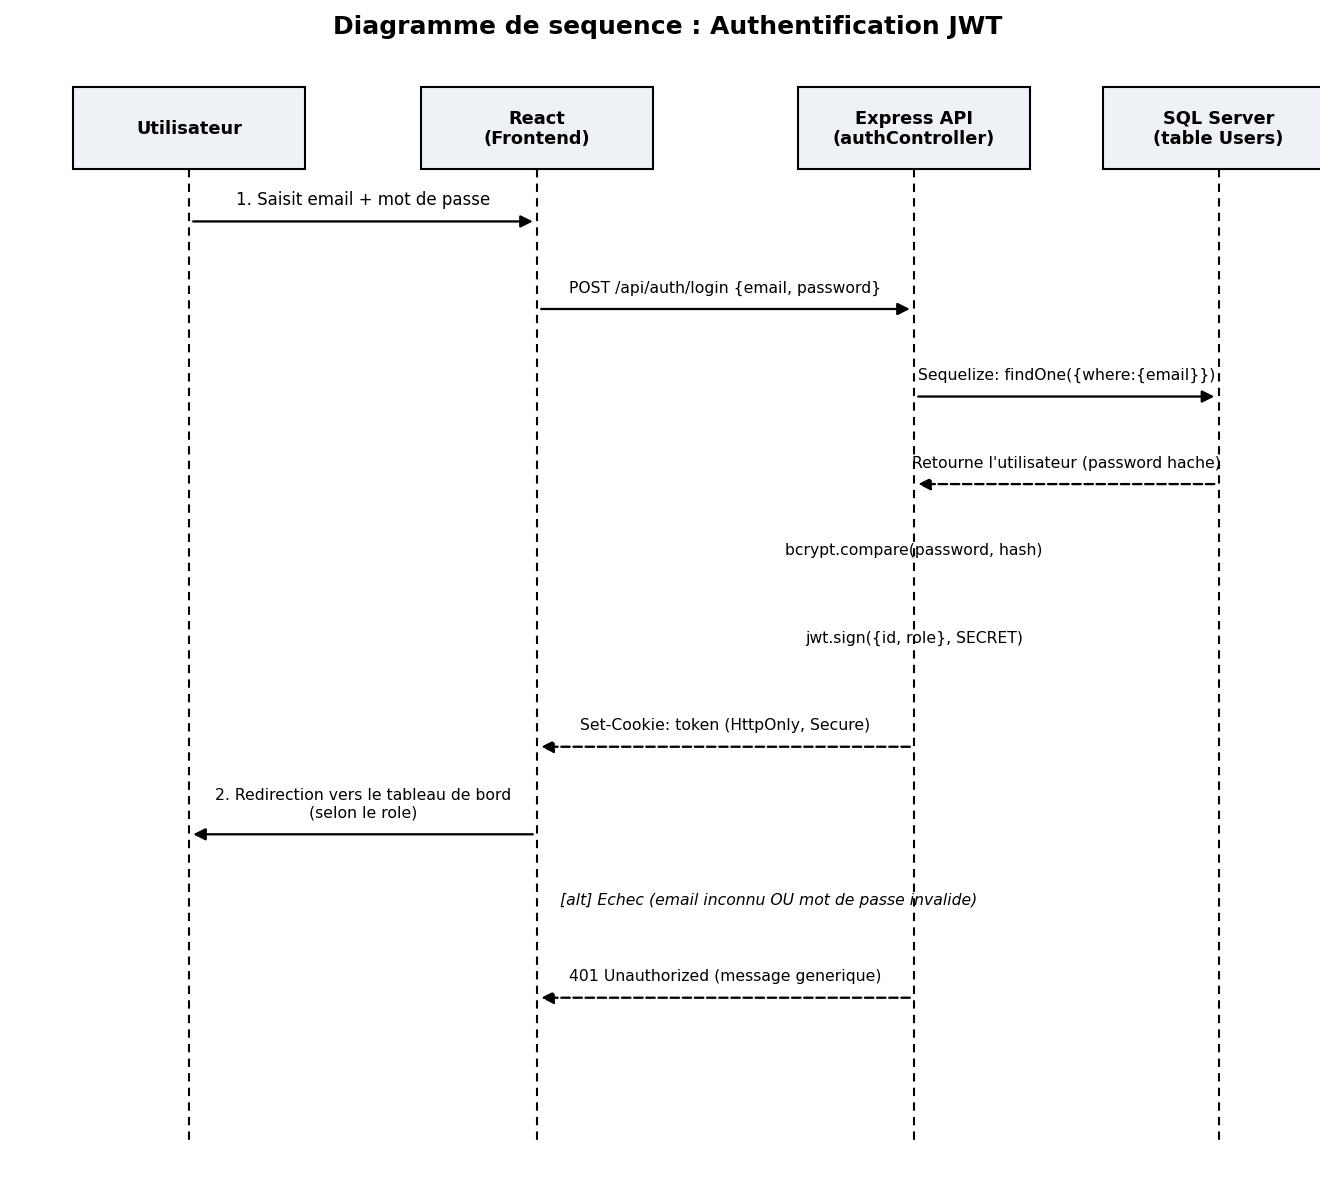
\includegraphics[width=0.8\textwidth]{img/DiagrammeSeqAuthentification.png}
    \caption{Diagramme de séquence du processus d'authentification JWT}
    \label{fig:seq_auth}
\end{figure}
\vspace{0.5cm}

\subsection{Le Tableau de Bord Administrateur (Admin Dashboard)}
Une fois authentifié en tant qu'Admin, l'utilisateur atterrit sur son espace dédié (Figure \ref{fig:dashboard_admin} et \ref{fig:home_page}). 

\vspace{0.5cm}
\begin{figure}[H]
    \centering
    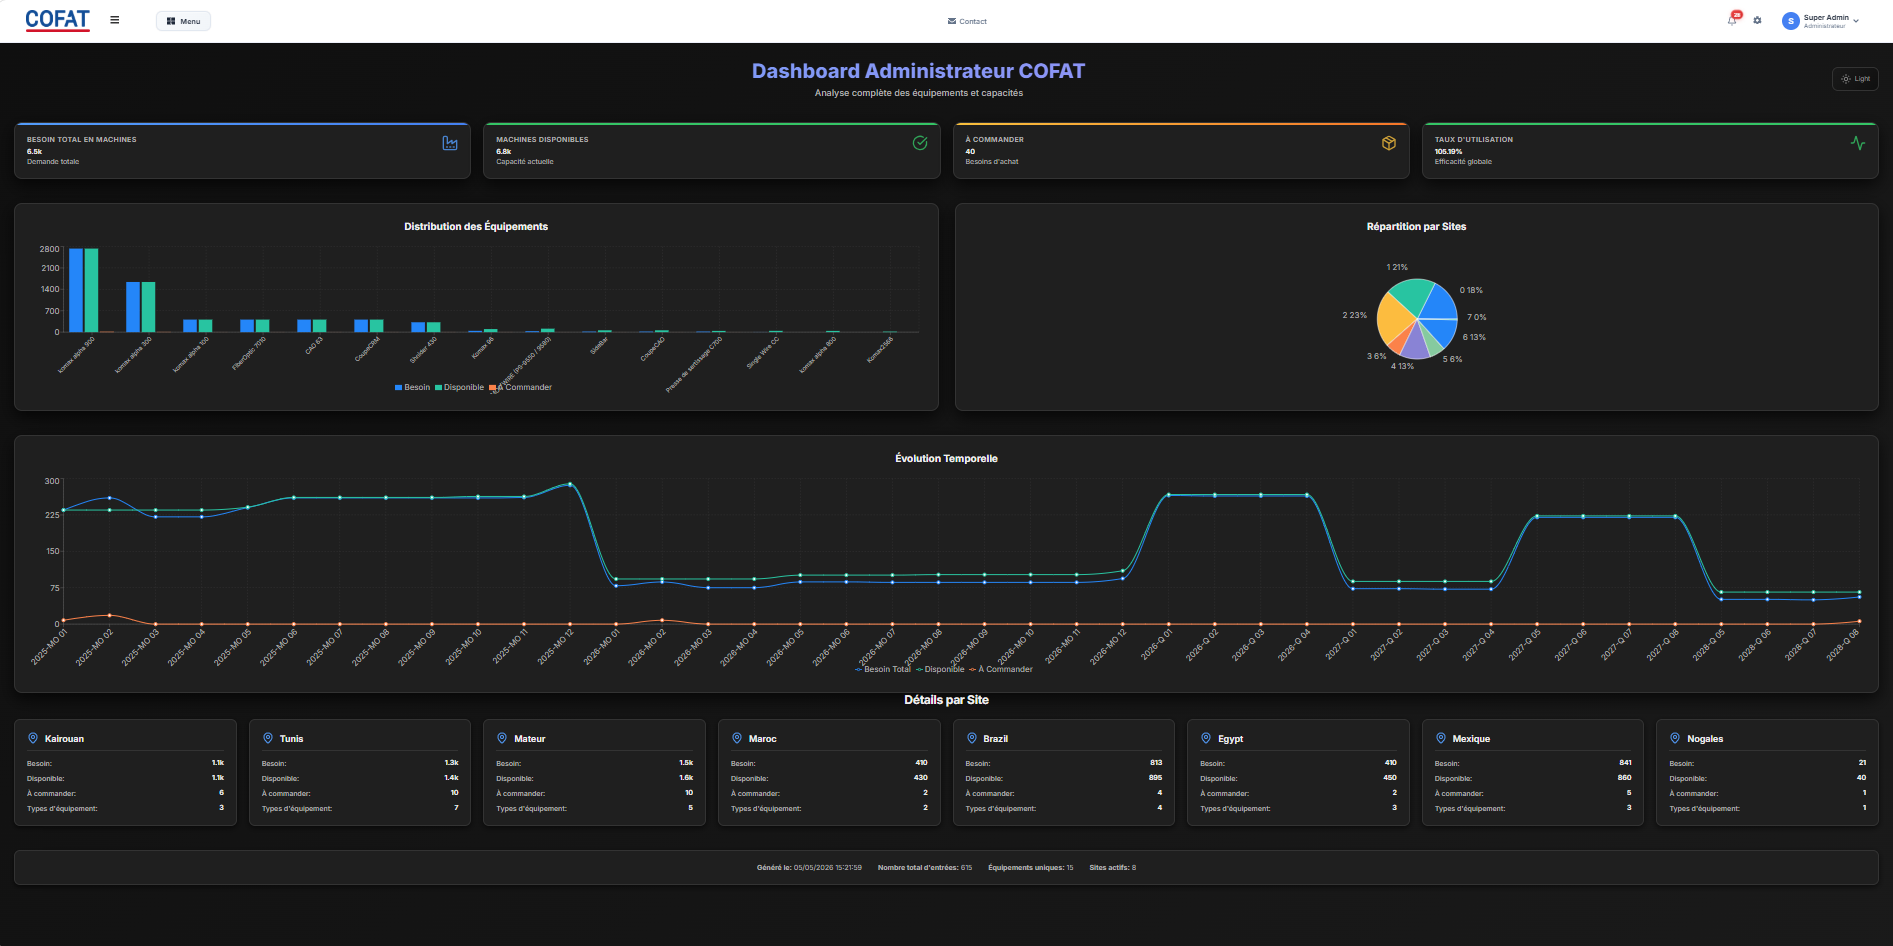
\includegraphics[width=0.8\textwidth]{img/dashboard admin.png}
    \caption{Tableau de bord de l'Administrateur}
    \label{fig:dashboard_admin}
\end{figure}
\vspace{0.5cm}

\vspace{0.5cm}
\begin{figure}[H]
    \centering
    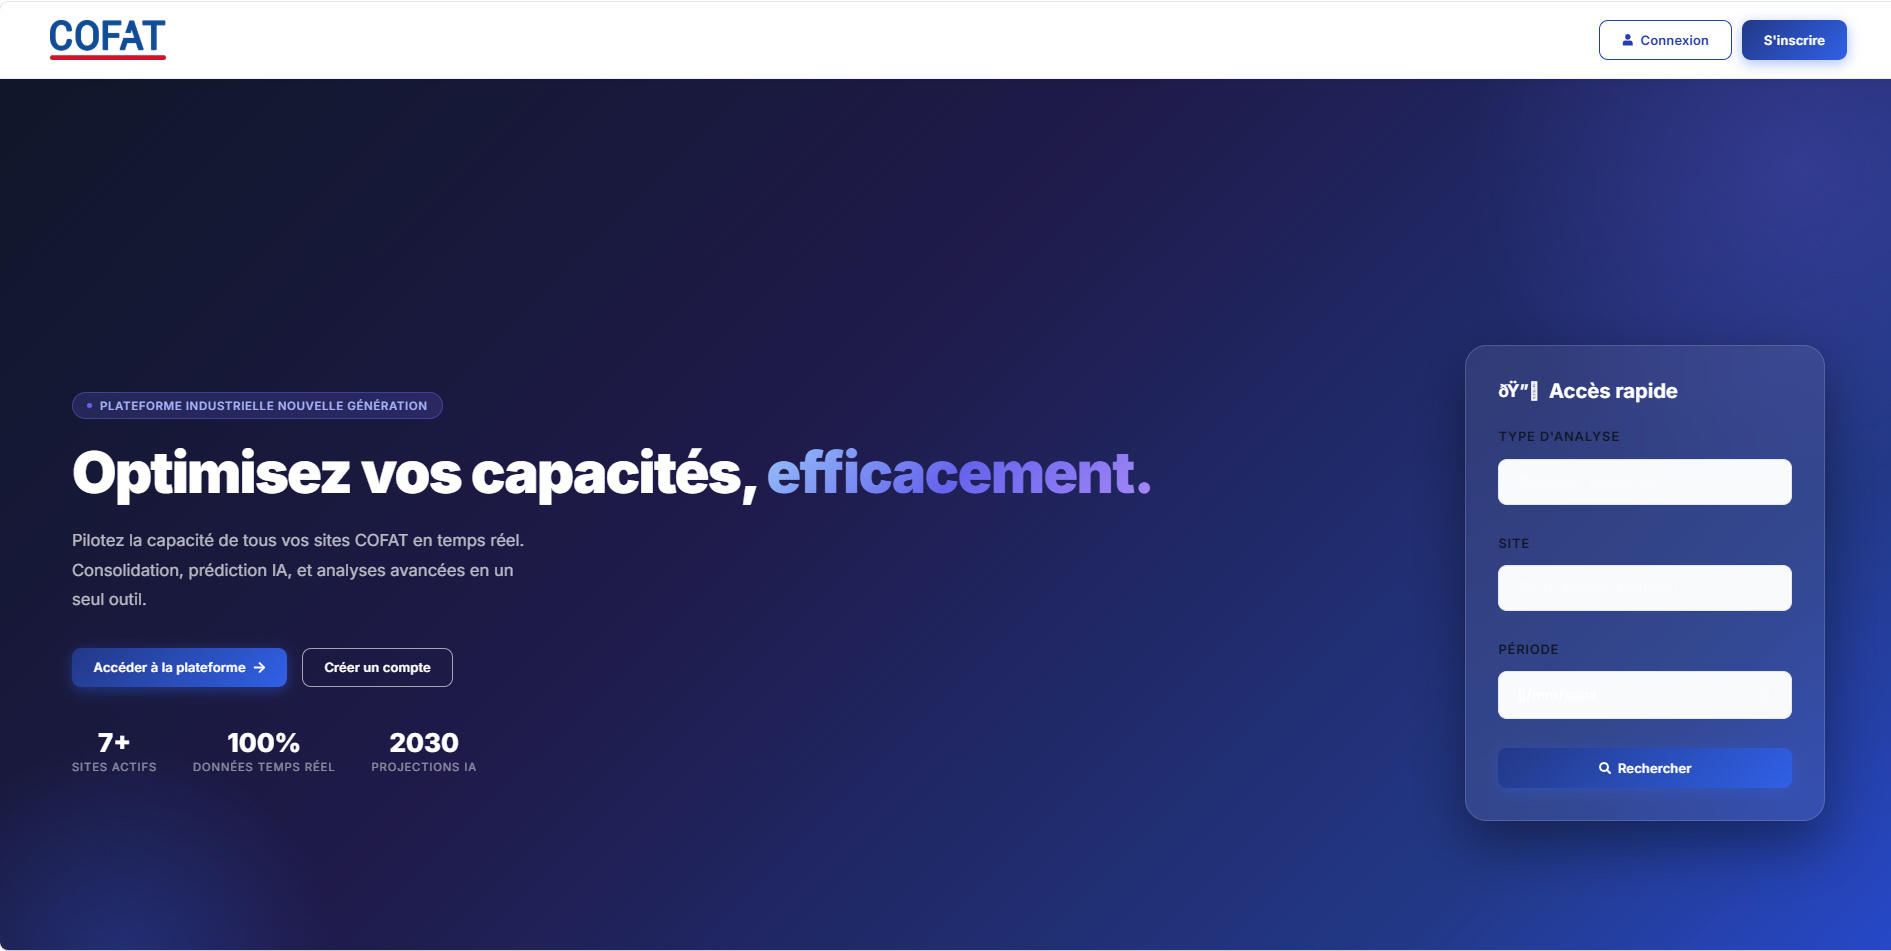
\includegraphics[width=0.8\textwidth]{img/HOME PAGE.png}
    \caption{Menu de navigation principal (Home Page)}
    \label{fig:home_page}
\end{figure}
\vspace{0.5cm}

\textbf{Description des fonctionnalités de l'interface :}
Le Dashboard est structuré de manière ergonomique avec une barre de navigation latérale (Sidebar) persistante. Depuis cet espace, l'Administrateur a accès aux modules vitaux du système :
\begin{itemize}
    \item \textbf{Gestion des Utilisateurs} : Un tableau CRUD permettant de créer des comptes pour les nouveaux ingénieurs, de leur assigner un mot de passe temporaire et de définir leur périmètre (Site de rattachement) et leur rôle strict (Admin, Site Manager, Achat).
    \item \textbf{Gestion des Sites} : Ajout de nouvelles entités industrielles (Code du site, pays, type) qui alimenteront dynamiquement les menus déroulants de toute l'application.
    \item \textbf{Accès aux Consolidations (Cofat Group)} : Raccourcis directs vers les vues mondiales des équipements et ressources humaines, affichant des tuiles de synthèse (KPIs) globales en haut de l'écran.
    \item \textbf{Catalogue StandardInvestment} : Accès centralisé au référentiel d'investissement du groupe.
\end{itemize}
La navigation est extrêmement fluide car il s'agit d'une SPA (Single Page Application) ; les composants React se montent et se démontent instantanément sans rafraîchissement global de la page web.

\textbf{Choix ergonomiques du Sprint 1 :} dès cette première itération fonctionnelle, une attention particulière a été portée à la cohérence visuelle de l'ensemble de l'application, condition indispensable pour une adoption rapide par des utilisateurs peu familiers des outils numériques métier. La palette de couleurs Tailwind CSS retenue reprend les teintes institutionnelles du Groupe COFAT, tandis que chaque module (Équipements, Espaces, RH, Budget) est identifié par une icône distincte issue de la bibliothèque \textit{lucide-react}, facilitant le repérage visuel rapide dans le menu latéral. Les temps de chargement des tableaux de bord ont également fait l'objet d'une vigilance dès ce sprint : des indicateurs de chargement (\textit{spinners}) et des états de type \textit{skeleton screen} ont été intégrés pour informer l'utilisateur qu'une requête est en cours, plutôt que de laisser l'écran statique pendant les quelques centaines de millisecondes nécessaires à l'agrégation des données par le serveur.

\subsection{Validation du Sprint 1}
La démonstration du Sprint 1 auprès du Product Owner, à l'issue du mois d'avril 2026, a permis de valider trois critères d'acceptation majeurs : la robustesse du mécanisme d'authentification (tentative de connexion avec des identifiants erronés correctement rejetée, jeton JWT expirant après la durée définie), l'étanchéité des rôles (un compte de test doté du rôle Site Manager ne pouvant pas accéder aux routes réservées à l'Admin, même en modifiant l'URL directement dans le navigateur), et l'ergonomie générale jugée satisfaisante par les utilisateurs pilotes du Backoffice de Tunis. Cette validation a ouvert la voie au développement des modules métier proprement dits, objets des chapitres suivants.


Un soin particulier a été apporté à la gestion des états transitoires de l'interface : chaque action asynchrone (chargement de la liste des utilisateurs, création d'un nouveau site) affiche un indicateur de chargement (\textit{spinner}) le temps que la réponse serveur soit reçue, et un message de confirmation ou d'erreur (\textit{toast}) s'affiche brièvement à l'écran une fois l'opération terminée, sans jamais bloquer l'interface ni forcer l'utilisateur à fermer une fenêtre modale d'alerte intrusive. Ce niveau de finition, bien qu'invisible dans le code métier proprement dit, contribue directement à l'adoption de l'outil par des utilisateurs non-informaticiens habitués jusque-là à la simplicité (et aux lenteurs) d'un fichier Excel.

\subsection{Validation du socle technique}
Avant de considérer le Sprint 1 comme clos, une phase de validation manuelle a été menée. Cette validation a couvert plusieurs scénarios critiques pour la suite du projet :
\begin{itemize}
    \item Tentative de connexion avec des identifiants erronés, afin de vérifier que le message d'erreur renvoyé par l'API ne divulgue pas d'information permettant de déduire si c'est l'email ou le mot de passe qui est incorrect (bonne pratique de sécurité contre l'énumération de comptes).
    \item Tentative d'accès direct à une route protégée (par exemple \texttt{/api/sites}) sans cookie JWT valide, confirmant le renvoi systématique d'un code HTTP 401.
    \item Vérification du comportement du cookie \textit{HttpOnly} via les outils de développement du navigateur, confirmant qu'aucun script JavaScript côté client ne peut lire ou manipuler le jeton, contrairement à un stockage classique en \texttt{localStorage}.
    \item Test de création, modification et suppression d'un utilisateur et d'un site depuis le Dashboard Admin, avec vérification croisée directe dans la base \texttt{GALIA\_V1} via SQL Server Management Studio.
\end{itemize}
Cette démarche de validation manuelle rigoureuse a permis de sécuriser la livraison de ce socle avant d'y adosser l'ensemble des modules métier développés lors des sprints suivants.

\section{Conclusion}
Au cours de ce chapitre, nous avons justifié et matérialisé l'architecture logicielle de \textit{Cofat Capacity Study}. Les choix de Node.js, Express, React et MS SQL Server apportent une robustesse et une évolutivité à la hauteur des enjeux de l'industrie automobile. La mise en place de l'architecture 3-tiers et le succès du Sprint 1 (déploiement du socle technique, sécurisation par JWT et interface d'administration) prouvent la viabilité technique de notre approche. 
Le socle étant désormais solidement en place, le chapitre 4 explorera en profondeur le cœur métier de la plateforme : le développement des interfaces de "Planification Locale" pour les usines (Sprint 2) et la prouesse algorithmique de la "Consolidation Groupe" en temps réel (Sprint 3).